 
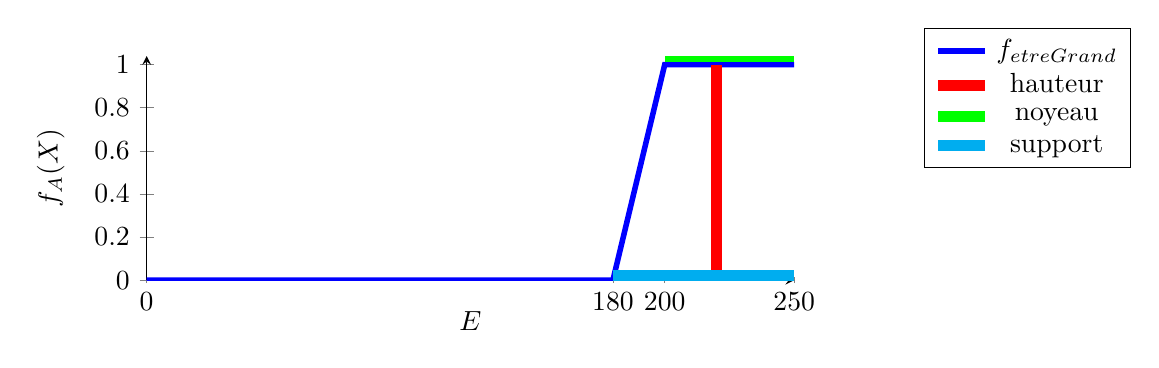
\begin{tikzpicture}
	\begin{axis}[
		xlabel={$E$},
		ylabel={$f_A(X)$},
		axis x line=bottom,
		axis y line=left,
		xscale=1.2,
		yscale=0.5,
		xtick=data,
		legend entries={$f_{etreGrand}$,hauteur,noyeau,support},
		legend style={at={(1,1)},anchor=south west}]
		
			\addplot+[mark=none,line width= 2] coordinates{(0,0)(180,0)(200,1)(250,1)};
			\addplot+[mark=none,line width= 4,red] coordinates{(220,0)(220,1)};
			\addplot+[mark=none,line width= 4,green] coordinates{(200,1.04)(250,1.04)};
			\addplot+[mark=none,line width= 4,cyan] coordinates{(180,0.02)(250,0.02)};
			
	\end{axis}	
\end{tikzpicture}